\documentclass[11pt]{book}
\usepackage{hyperref}
\usepackage{textcomp}
\usepackage{colonequals}
\usepackage{amsfonts}
\usepackage{amssymb}
\usepackage{amsmath}
\usepackage[utf8]{inputenc}
\usepackage[T1]{fontenc}
\usepackage{float}
\usepackage{fixltx2e}
\usepackage[italian]{babel}
\usepackage{graphicx}

\newenvironment{sistema}%
{\left\lbrace\begin{array}{@{}l@{}}}%
{\end{array}\right.}


\title{Appunti di Ricerca Operativa}
\author{Fabio Viola}
\date{}

\setcounter{chapter}{10}

\begin{document}

\chapter{Simulazione discreta}

\scriptsize {\bf Slide}:
\href{http://www.or.deis.unibo.it/staff_pages/martello/Chapter11.zip}{Discrete
  Simulation} \normalsize
\vspace{20pt}

Nel primo capitolo abbiamo fatto un esempio di un problema
affrontabile con metodologie di ricerca operativa, quello
dell'ottimizzazione del front office. Ad uno sportello si vuole
ridurre il personale mantenendo un'appropriata qualit\`a del
servizio. Un simile problema \`e affrontabile con metodologie
provenienti dalla teoria delle code, tuttavia quando il sistema in cui
si gestiscono code d'attesa \`e dinamico (cio\`e le sue
caratteristiche variano nel tempo) e quando vi \`e un gran numero di
entit\`a, l'unico strumento utilizzabile \`e la {\bf simulazione}.

In cosa consiste la simulazione? La simulazione consiste nel creare un
modello in cui il sistema viene suddiviso in un insieme di elementi
aventi vita indipendente, dotati di particolari caratteristiche e
collegati da relazioni. Il sistema subisce delle trasformazioni in
seguito agli eventi. La simulazione ci consente di studiare
l'evoluzione del sistema e verificare i valori dei parametri
statistici che siamo interessati a valutare.

Per introdurre un p\`o di terminologia possiamo chiamare:

\begin{itemize}
\item {\bf entit\`a}: gli elementi del sistema aventi vita
  indipendente;
\item {\bf attributi}: le caratteristiche di ogni entit\`a;
\item {\bf insiemi} o {\bf code}: le relazioni che collegano due o
  pi\`u entit\`a;
\item {\bf eventi}: attivit\`a che producono variazioni nel sistema.
\end{itemize}

Il risultante programma di simulazione viene eseguito con {\bf valori
  casuali} per generare eventi simulati nel tempo secondo delle {\bf
  distribuzioni di probabilit\`a}.

Esistono due modalit\`a di simulazione: quella {\bf discreta} e quella
{\bf continua}. Noi siamo interessati alla prima in quanto \`e quella
pi\`u importante e frequentemente utilizzata in termini industriali e
ingegneristici. La seconda \`e utilizzata ad esempio per realizzare
uno studio di fenomeni metereologici o nucleari.

Un programma di simulazione viene strutturato tenendo presente due parti:

\begin{itemize}
\item {\bf struttura statica}: composta da entit\`a, attributi e code;

\item {\bf struttura dinamica}: costituita dagli eventi che modificano
  lo stato del sistema.
\end{itemize}

Sono questi due componenti ceh consentono di realizzare un programma
scritto in un determinato linguaggio di programmazione per realizzare
la simulazione. Il linguaggio pi\`u utilizzato anni fa era {\bf
  Simula67} (dove 67 identifica l'anno in cui \`e stato
inventato!). Oggi questo linguaggio (che \`e uno dei primissimi
linguaggi ad oggetit) non \`e pi\`u utilizzato, ma vedremo quali
vengono adoperati.

\section{Generazione di valori pseudo-casuali}

Nei modelli di simulazione ha un ruolo cruciale la generazione di
valori casuali secondo una determinata {\bf distribuzione di
  probabilit\`a}. Spesso si utilizzano sistemi per generare dei numeri
casuali che in realt\`a risultano addirittura essere deterministici in
quanto partendo da un seme iniziale determinano il risultato
sfruttando un algoritmo. Questi numeri li chiamiamo {\bf
  pseudo-casuali} ed in molti casi possono essere equiparati a numeri
casuali.

Riprendiamo ora dei concetti del mondo della probabilit\`a che ci
torneranno utili a breve. Sia {\em x} una {\bf variabile aleatoria} ed
indichiamo con {\em t} un {\em evento} di {\em x}. Definiamo {\bf
  funzione densit\`a di probabilit\`a} la seguente funzione:

\begin{center}
$f(x) = \lim\limits_{\Delta x \rightarrow 0} \frac{\mathbb{P}(x \leq t
    \leq x + \Delta x)}{\Delta x}$
\end{center}

dove $\mathbb{P}(A)$ indica la probabilit\`a dell'evento {\em A} (per
cui $f(x)\geq 0$ per ogni $x$). Preso un valore {\em x} e preso un
intervallo $\Delta x$, il valore di $f(x)$ \`e la probabilit\`a che
{\em t} cada l\`i dentro, divisa per $\Delta x$.

Sapendo ci\`o, calcolando l'integrale da {\em a} a {\em b}, questo ci
dar\`a la probabilit\`a che un valore sia compreso fra {\em a} e {\em
  b}:

\begin{center}
$\int\limits_{a}^b f(x)dx = P(a\leq t \leq b)$  
\end{center}

Portando gli intervalli agli estremi ponendo $a = \-infty$ e $b =
+\infty$ otteniamo la cosiddetta {\bf condizione di normalizzazione}:

\begin{center}
$\int\limits_{-\infty}^{+\infty} f(x)dx = 1$
\end{center}

Dalla densit\`a di probabilit\`a possiamo ricavare altre funzioni
interessanti:

\begin{itemize}
\item il {\bf valore atteso} (o {\bf speranza}): $\mathbb{E} =
  \int\limits_{-\infty}^{+\infty} f(x)x\phantom{,}dx$

\item la {\bf varianza}: $V = \sigma^2 = \int\limits_{-\infty}^{+\infty}
  f(x)(x-E)^2\phantom{,}dx$

\item la {\bf funzione di distribuzione cumulativa}: $F(x) =
  \int\limits_{-\infty}^{x} f(\xi)d\xi = \mathbb{P}(t\leq x)$

  Questa funzione, sulla base della sua definizione, \`e monotona
  crescente e soddisfa $0 \leq F \leq 1$. Questa funzione \`e quella
  che viene utilizzata per generare dei valori aventi una qualunque
  distribuzione di probabilit\`a (partendo da valori uniformemente
  distribuiti fra 0 e 1), infatti:
  
  {\bf Teorema}: se si generano valori {\em r} uniformemente
  distribuiti fra 0 e 1, i corrispondenti valori $F^{-1}(r)$ hanno
  funzione di densit\`a di probabilit\`a $f(x)$.

  \vspace{11pt}
  $\square$ {\bf Dimostrazione}: per una variabile aleatoria {\em y}
  uniformemente distribuita fra 0 e 1 si ha evidentemente $f(y) = 1
  \forall y\quad (0\leq y \leq 1)$. Pertanto:
  
  \begin{center}
    $\mathbb{P}(r \leq q) = \int\limits_{0}^q f(\xi)d\xi = q \quad
    \forall q : (0 \leq q \leq 1)$
  \end{center}

  da cui in particolare, dato un valore {\em x}, si ha $\mathbb{P}(r
  \leq F(x)) = F(x)$. Si osservi ora che (vedere figura
  \ref{cap11fig1}) $\mathbb{P}(r \leq F(x)) = \mathbb{P}(F^{-1}(r)\leq
  x)$ per cui dall'integrale visto poco fa, $F(x) =
  \mathbb{P}(F^{-1}(r) \leq x)$. Abbiamo quindi dimostrato che la
  funzione $F^{-1}(r)$ ha funzione di distribuzione cumulativa data da
  $F(x)$, ossia la funzione densit\`a di probabilit\`a \`e proprio
  $f(x)$. $\blacksquare$
  \vspace{11pt}

  \begin{figure}{H}
  \centering
  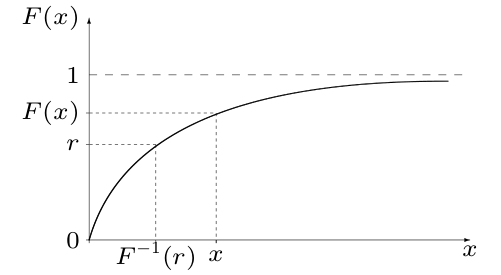
\includegraphics[width=0.65\textwidth]{images/cap11fig1.png}
  \caption{Funzione di distribuzione cumulativa}
  \label{cap11fig1}
  \end{figure}

\end{itemize}

Vediamo adesso alcuni esempi.

\vspace{11pt} $\blacktriangleright$ {\bf Esempio}: vogliamo generare
valori aventi funzione densit\`a di probabilit\`a $f(x) = 8x$ per $0
\leq x \leq \frac{1}{2}$. Possiamo scrivere la funzione di
distribuzione cumulativa $F(x)$:

\begin{center}
$F(x) = \int\limits_{-\infty}^{x} f(\xi) d\xi$
\end{center}

Il valore $-\infty$ pu\`o essere sostituito con $0$ in quanto sappiamo
che la funzione densit\`a di probabilit\`a \`e limitata
nell'intervallo $[0,\frac{1}{2}]$:

\begin{center}
$\int\limits_{0}^x 8\xi d\xi = 8 \biggr[\frac{\xi^2}{2}\biggr]_0^x =
  4x^2$
\end{center}

Abbiamo anche sostituito a $f(x)$ il valore $8x$ che corrisponde alla
densit\`a di probabilit\`a fornitaci dal testo.

A questo punto possiamo porre $r = 4x^2$ e ricavare $x =
\frac{\sqrt{r}}{2}$. Baster\`a generare valori compresi fra 0 e 1 per
ottenere dei valori distribuiti secondo la densit\`a di probabilit\`a
assegnata. $\blacktriangleleft$
\vspace{11pt}

\vspace{11pt} $\blacktriangleright$ {\bf Esempio}: {\bf distribuzione
  uniforme}. In molti casi si ha a che fare con valori che possono
essere simulati con una distribuzione uniforme fra un valore minimo
{\em a} ed un valore massimo {\em b}. Osserviamo a questo proposito la
figura \ref{cap11fig2}.

\begin{figure}[H]
  \centering
  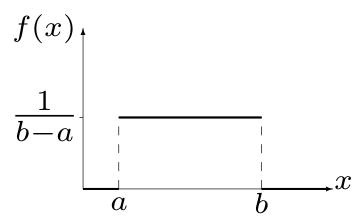
\includegraphics[width=0.4\textwidth]{images/cap11fig2.png}
  \caption{Distribuzione uniforme}
  \label{cap11fig2}
\end{figure}

In questi casi si ha:

\begin{center}
$f(x) = \frac{1}{b-a}(a \leq x \leq b)$  
\end{center}

da cui:

\begin{center}
$F(x) = \int\limits_{a}^b \frac{1}{b-a}d\xi = \frac{1}{b-a}\bigr[\xi \bigr]_a^\xi
  = \frac{x-a}{b-a}$  
\end{center}

Ponendo $r = \frac{x-a}{b-a}$, si ottiene $x = a+r(b-a)$. Questo
corrisponde a sommare ad {\em a} una frazione casuale dell'intervallo
$[a,b]$. Il valor medio di tale distribuzione \`e:

\begin{center}
$\mathbb{E} = \int\limits_{a}^b \frac{x}{b-a}dx = \frac{1}{b-a}
  \biggr[ \frac{x^2}{2} \biggr]_a^b = \frac{1}{b-a} \cdot
  \frac{b^2-a^2}{2} = \frac{a+b}{2}$ $\quad\blacktriangleleft$
\end{center}
\vspace{11pt}

\vspace{11pt}
$\blacktriangleright$ {\bf Esempio}: {\bf distribuzione
  esponenziale}. Una distribuzione esponenziale di parametro $\lambda$
ha funzione densit\`a di probabilit\`a come in figura \ref{cap11fig3}.

\begin{figure}[H]
  \centering
  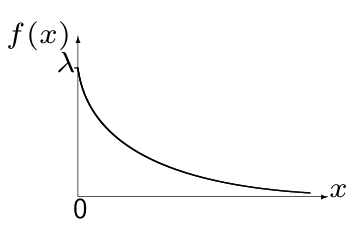
\includegraphics[width=0.4\textwidth]{images/cap11fig3.png}
  \caption{Distribuzione esponenziale}
  \label{cap11fig3}
\end{figure}

Per tale distribuzione:

\begin{itemize}
\item il {\bf valor medio} \`e: $\mathbb{E} = \frac{1}{\lambda}$;
\item la varianza \`e $V = \sigma^2 = \frac{1}{\lambda^2}$
\item la funzione di distribuzione cumulativa \`e:
\begin{center}
 $F(x) = \int\limits_{0}^x \lambda e^{-\lambda \xi} d\xi = \lambda
  \biggr[ - \frac{e^{-\lambda \xi}}{\lambda} \biggr]_0^{x} =
  1-e^{-\lambda x}$
\end{center}
\end{itemize}

Ponendo $r = 1-e^{-\lambda x}$, si ha $1-r = e^{-\lambda x}$. Non \`e
facile ricavare la {\em x}, dunque si pone $r' = 1-r$ e possiamo
scrivere cos\`i $r' = e^{-\lambda x}$, quindi $ln(r') = -\lambda x$.

Perch\'e \`e cos\`i importante la distribuzione esponenziale? Perch\'e
i processi di Poisson sono molto utilizzati per modellare arrivi
casuali dei clienti in una coda. $\lambda$ \`e il numero medio di
arrivi durante un'unit\`a di tempo. L'intervallo di tempo fra due
eventi consecutivi segue sempre una distribuzione esponenziale di
valor medio $\frac{1}{\lambda}$ ({\bf importante!}).
$\blacktriangleleft$
\vspace{11pt}

\section{Primi esempi di modelli di simulazione}

Vediamo il primo esempio: una stazione di servizio con una sola pompa
di benzina. Supponiamo che gli arrivi dei clienti seguano una
distribuzione di Poisson con un valor medio $\lambda$ e che il tempo
di rifornimento sia uniformemente distribuito fra due valori $T1$ e
$T2$. Se ci sono $NMAX$ clienti in coda, chi arriva si arrende e se ne
va. La simulazione la fermiamo quando arrviamo a {\em NTOT} clienti
completati, dove con completati intendiamo che arrivano, vengono
riforniti e vanno via. Questo ci permette di eliminare delle
impurit\`a dai dati dovute a clienti non completati.

\begin{figure}[H]
  \centering
  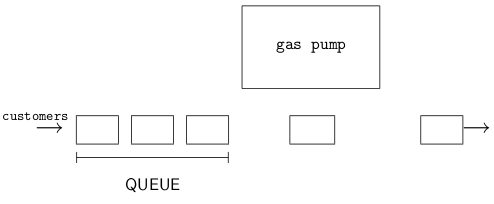
\includegraphics[width=0.8\textwidth]{images/cap11fig4.png}
  \caption{Stazione di servizio}
  \label{cap11fig4}
\end{figure}

La descrizione statica viene realizzata studiando lo stato del
sistema. Quali sono i principali oggetti di un modello di simulazione?
Lo vediamo nella seguente schematizzazione:

\vspace{11pt}
\begin{tabular}{lp{4cm}p{4cm}}
{\bf Terminologia} & {\bf Esempi} & {\bf SIMSCRIPT} \\\hline
{\em Entit\`a} & auto & AUTO \\
{\em Generazione} & genera l'auto & CREATE AUTO \\ 
{\em Distruzione} & distruggi l'auto & DESTROY AUTO \\\hline
{\em Attributi} & istante di ingresso in coda & TIC(AUTO) \\\hline
{\em Insiemi} & coda & CODA \\
& inserisci l'auto in coda & FILE AUTO IN CODA \\
& estrai la prima auto dalla coda & REMOVE FIRST AUTO FROM
CODA\\\hline
{\em Eventi} & innesca un evento Fine servizio con ritardo T &
SCHEDULE AN F.SERV AT TIME.V + T\\\hline
\end{tabular}
\vspace{11pt}

In questa tabella abbiamo inserito nell'ultima colonna la sintassi
SIMSCRIPT che \`e un potentissimo ed utilizzatissimo linguaggio per le
simulazioni.

% Appunti Alessandra 09/05/12

Dunque abbiamo delle {\bf entit\`a} che sono dotate di {\bf
  attributi}. E l'altro oggetto importante sono le {\bf
  code}. Concentriamoci ora sulla creazione e sulla distruzione delle
entit\`a. Per ogni entit\`a bisogna memorizzare delle informazioni,
pertanto ogni entit\`a ha bisogno di un'area di memoria allocata, in
cui vengono memorizzate le informazioni iniziali delle entit\`a e le
informazioni via via raccolte nel corso della simulazione. In un
modello complesso, in cui ci sono molte entit\`a, si ha bisogno di un
numero elevato di aree di memoria. Tornando all'esempio delle auto
alla stazione di servizio, finch\'e un'auto \`e nel sistema (cio\`e \`e in
coda, o alla stazione di servizio) serve che siano mantenute tutte le
informazioni su di essa. Quando poi esce dal sistema, i dati di cui
avevamo bisogno per fare le considerazioni statistiche li abbiamo
tutti, quindi le informazioni su quell'auto non servono pi\`u e possono
essere rimosse. Dunque si fa uso dell'allocazione dinamica della
memoria. \`E importante rimuovere le entit\`a in quanto in sistemi molto
complessi la memoria verrebbe altrimenti subito riempita. Quindi
ricapitolando: all'entrata nel sistema abbiamo un'istruzione di alto
livello ``CREATE CAR'' che riserver\`a un'area di memoria libera di
dimensioni opportune; quest'area viene conservata finch\'e l'auto non
esce dal sistema, e solo a quel punto ci sar\`a l'istruzione ``DESTROY
CAR'' che comunica al sistema che l'area \`e stata liberata.

Passiamo ora alla {\bf descrizione dinamica del sistema}. L'elemento
fondamentale per la gestione dinamica \`e il {\bf tempo simulato}. Nei
primi linguaggi di simulazione esso veniva realizzato mediante un
contatore che, ad ogni incremento di un'unit\`a di tempo, verificava
l'esistenza di cambiamenti dello stato del sistema. Cio\`e \`e come se
in ogni istante venisse fatta una fotografia del sistema per vedere se
qualcosa era cambiata rispetto all'istante precedente. Nei moderni
linguaggi di simulazione invece, non si considerano tutti gli istanti
di tempo, ma solo quelli in cui il sistema deve cambiare, e si manda
in esecuzione la parte di programma contenente le istruzioni da
eseguire in quell'istante. Nell'esempio delle auto lo stato del
sistema cambia ad esempio quando {\em arriva un'auto} o {\em termina
  il servizio di un'auto}.

Per la modellazione della dinamica di un sistema esistono diversi
approcci: noi useremo quello della {\bf programmazione degli eventi} o
{\bf schedulazione degli eventi}. L'{\bf evento} \`e il sottoprogramma
da eseguire nell'istante in cui cambia lo stato del sistema, cio\`e
quando si verifica l'evento. Quando un evento termina, il sistema deve
sapere in qualche modo qual \`e il prossimo evento da eseguire. C'\`e
bisogno quindi, durante l'esecuzione di un evento, di avere
un'istruzione che comunichi al sistema quale evento deve avvenire in
futuro e in quale istante. Quindi in ogni evento vengono determinati
gli eventuali eventi che devono avvenire in futuro e li si {\em
  innesca}. Al termine dell'esecuzione di un evento, il sistema (che
avr\`a a disposizione una coda degli eventi futuri, con i relativi
ritardi) determina il prossimo evento da eseguire ed aggiorna il tempo
simulato. 

Per individuare quali sono gli eventi necessari \`e utile costruire un
{\em diagramma temporale} nel quale si considerano tutte le possibili
situazioni in cui cambia lo stato del sistema. Riprendiamo l'esempio
della stazione di servizio e indichiamo con $A_i$ l'arrivo dell'auto
i-esima, con $S_i$ l'istante di inizio del servizio dell'auto i-esima,
e con $E_i$ la fine di tale servizio. Assumiamo inoltre che in coda
possano esserci al massimo $N_{MAX}=2$ auto, e che quindi se arriva
un'auto e trova la coda piena va via. Facciamo quest'assunzione in
modo che tutte le possibili situazioni si verifichino in tempi
brevi. Ecco un esempio di evoluzione temporale del sistema sull'asse
del tempo:

\begin{figure}[H]
  \centering
  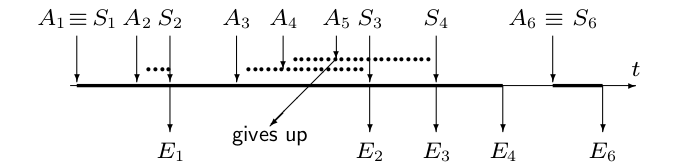
\includegraphics[width=0.8\textwidth]{images/cap11fig5.png}
\end{figure}

I tratti in cui l'asse temporale \`e in grassetto sono gli intervalli
in cui la stazione \`e impegnata. I puntini indicano che un'auto si \`e
messa in coda, mentre se ci sono due auto in coda abbiamo due strati
di puntini. Ogni modello di simulazione deve prevedere un'evento
iniziale che avvii l'esecuzione, inizializzando il sistema e
innescando nel nostro caso l'arrivo di un'auto (con un ritardo pari a
zero). La struttura del modello \`e rappresentata mediante il {\bf
  diagramma degli inneschi}:

\begin{figure}[H]
  \centering
  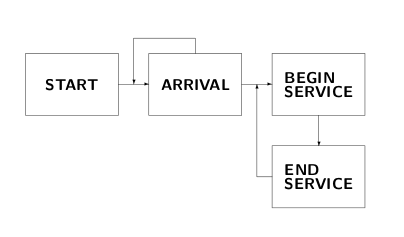
\includegraphics[width=0.6\textwidth]{images/cap11fig6.png}
\end{figure}

In questo schema abbiamo gli eventi, tra cui l'evento iniziale, e ogni
freccia sta ad indicare la {\bf possibilit\`a} che un evento inneschi
un altro evento (non \`e detto che poi lo inneschi sempre).
 
Descriviamo il diagramma. Quando arriva un'auto siamo in grado di
stabilire quando arriver\`a la prossima, in quanto sappiamo che le auto
arrivano secondo una distribuzione esponenziale di valor medio
$1/\lambda$ (corrispondente al processo di Poisson di valor medio
$\lambda$). Quindi l'evento ``arrivo'' innesca il successivo
``arrivo'' con un ritardo casuale $T$ calcolato a partire da tale
distribuzione. Ecco perch\'e c'\`e la freccia dall'evento ``arrivo''
all'evento ``arrivo''. Inoltre vi \`e la freccia tra l'evento
``arrivo'' e l'evento ``inizio servizio'': questo perch\'e, se la
stazione \`e libera, l'arrivo di un'auto innesca l'inizio del servizio
con un ritardo pari a zero. Altrimenti l'auto entrer\`a in
coda. L'evento ``inizio servizio'' innesca sicuramente l'evento ``fine
servizio'', e infine la fine del servizio innesca (se c'\`e qualcuno in
coda) l'inizio del servizio di un'altra auto. Quindi come vediamo le
frecce non implicano un innesco sicuro, ma solo un possibile innesco.

Iniziamo a vedere quali istruzioni devono essere eseguite per ogni
evento che avviene, attraverso i {\em diagrammi di flusso} degli
eventi. Il primo che vediamo \`e quello in figura \ref{cap11fig7}. Il
simbolo $S$ indica l'ingresso nell'evento, mentre $R$ indica l'uscita.

\begin{figure}[h!]
  \centering
  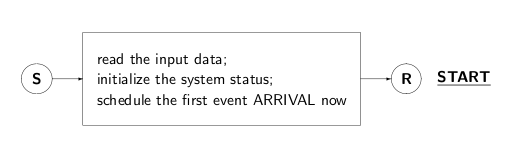
\includegraphics[width=0.7\textwidth]{images/cap11fig7.png}
  \caption{L'evento {\em start}}
  \label{cap11fig7}
\end{figure}

Alla fine di questo evento il sistema vede quale evento \`e stato
innescato: \`e stato innescato l'evento ``arrivo'' (figura
\ref{cap11fig8}).

\begin{figure}[h!]
  \centering
  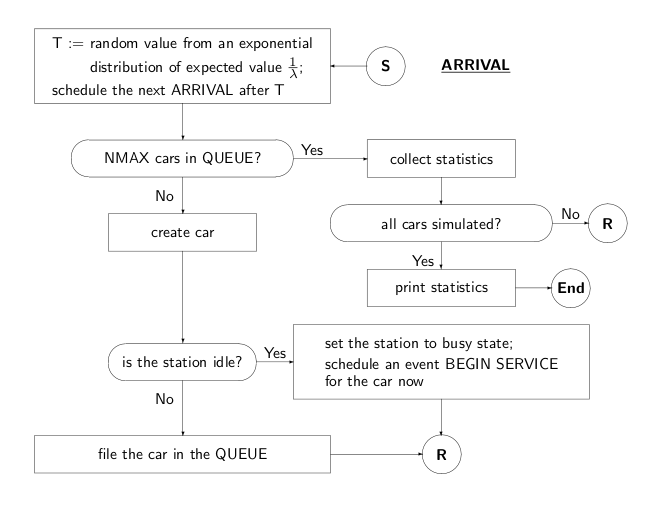
\includegraphics[width=\textwidth]{images/cap11fig8.png}
  \caption{L'evento {\em arrivo}}
  \label{cap11fig8}
\end{figure}

Che procedura viene attivata all'arrivo di un'auto? Prima di tutto,
come vediamo dal diagramma di flusso, viene calcolato il ritardo $T$
con il quale arriver\`a un'altra auto, e viene innescato l'arrivo di
tale auto. Poi si controlla se la coda \`e piena. 

Se \`e piena, l'auto deve uscire dal sistema, quindi si raccolgono i
dati per le statistiche (ad esempio per le statistiche relative alle
auto che rinunciano ad entrare). Poi bisogna controllare se \`e stato
raggiunto il numero di auto da simulare completamente (perch\'e
vogliamo terminare la simulazione dopo che un certo numero di auto \`e
stato simulato completamente, ovvero \`e entrato e uscito dal sistema):
quindi se l'auto in questione \`e l'ultima, allora si stampano in
output le statistiche e la simulazione termina completamente
(``END''). Altrimenti l'auto uscir\`a semplicemente dal sistema ma la
simulazione continuer\`a. 

Se invece la coda non \`e piena, viene creata l'entit\`a {\em auto}
(cio\`e si alloca un'area di memoria opportuna), e poi si controlla se
la stazione \`e libera: se non \`e libera l'auto verr\`a messa in coda e
finisce l'evento, altrimenti la stazione viene occupata, e viene
innescato l'evento ``inizio servizio'' per l'auto in questione, senza
ritardo. E l'evento ``arrivo'' finisce qui.

A questo punto inizia l'esecuzione dell'evento innescato, ``inizio
servizio'' \ref{cap11fig9}. Non si fa altro che calcolare un valore
random a partire dalla distribuzione uniforme nell'intervallo
$[T1,T2]$: questo valore sar\`a il tempo necessario per servire l'auto
corrente, e quindi verr\`a innescato l'evento ``fine servizio'' con un
ritardo pari proprio a $T$.

Nell'evento ``fine servizio'' (figura \ref{cap11fig9}) vengono
raccolti i dati statistici e poi viene liberata l'area di memoria
allocata per l'auto corrente. Poi se tutte le auto sono state simulate
completamente (cio\`e se si \`e raggiunto il numero di auto che si
voleva simulare) si stampano i dati statistici e si termina la
simulazione. Altrimenti si vede se c'\`e qualcuno in coda: se c'\`e
qualcuno in coda si estrae dalla coda la prima auto e si innesca
immediatamente l'evento ``inizio servizio'', altrimenti si indica che
la stazione \`e libera. Cos\`i termina l'evento ``fine servizio''.

\begin{figure}[H]
  \centering
  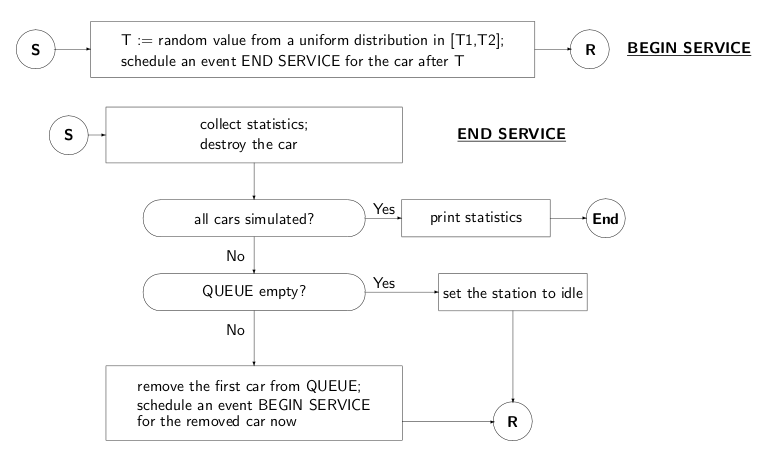
\includegraphics[width=\textwidth]{images/cap11fig9.png}
  \caption{L'evento {\em fine servizio}}
  \label{cap11fig9}
\end{figure}

Facciamo ora una considerazione importante che ci consentir\`a di
rendere pi\`u leggibili ed efficienti i modelli. Notiamo che l'evento
``inizio servizio'' coincide sempre temporalmente o con un evento
``arrivo'' o con un evento ``fine servizio''. Per cui possiamo
semplificare il modello eliminando tale evento inutile, e innescando
direttamente l'evento ``fine servizio'' nei due punti in cui veniva
innescato l'evento ``inizio servizio''. 

\begin{figure}[H]
  \centering
  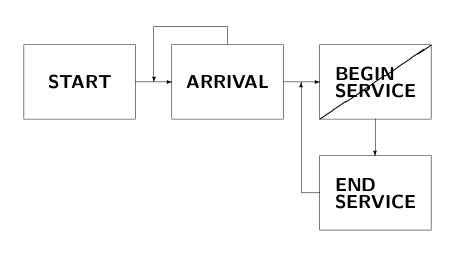
\includegraphics[width=0.55\textwidth]{images/cap11fig10.png}
\end{figure}

Quindi in generale si cerca di eliminare gli {\bf eventi inutili},
ovvero quegli eventi che coincidono sempre temporalmente con uno o
pi\`u altri eventi. Questo perch\'e l'innesco di un evento comporta
l'esecuzione di procedure molto pesanti per il sistema, il quale deve
aggiornare le sue strutture dati per stabilire come collocare tale
evento. Nel nostro esempio sostituiamo nell'evento ``arrivo'' il
blocco eseguito nel caso di stazione libera con un nuovo blocco come
in figura \ref{cap11fig11}.

\begin{figure}[h!]
  \centering
  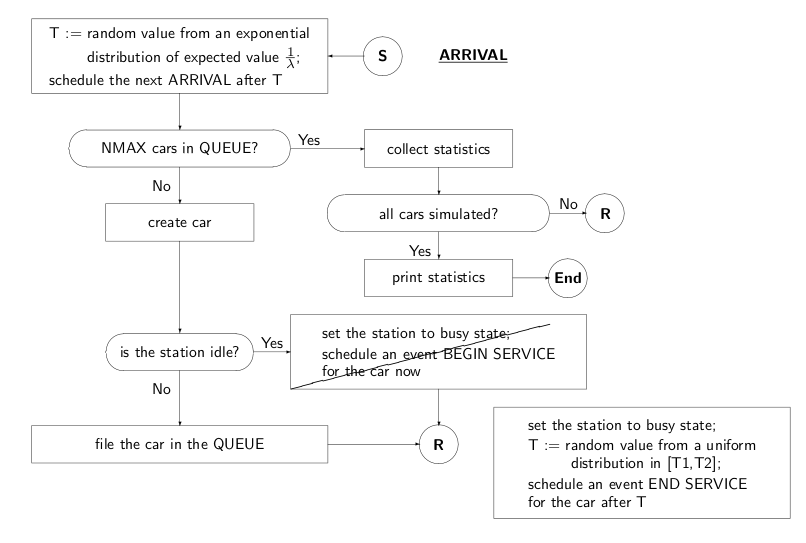
\includegraphics[width=\textwidth]{images/cap11fig11.png}
  \caption{Il nuovo evento {\em arrivo}}
  \label{cap11fig11}
\end{figure}

quindi se la stazione \`e libera, si occupa la stazione, ma invece di
innescare immediatamente l'evento ``inizio servizio'' che poi
innescher\`a l'evento ``fine servizio'', si innesca direttamente
l'evento ``fine servizio'' dopo un ritardo $T$ random calcolato a
partire dalla distribuzione uniforme nell'intervallo $[T1,T2]$.

Inoltre non ci sar\`a pi\`u l'evento ``inizio servizio'', mentre
nell'evento ``fine servizio'' sostituiamo il blocco eseguito nel caso
in cui la coda non sia vuota, con un nuovo blocco (figura
\ref{cap11fig12}).

\begin{figure}[H]
  \centering
  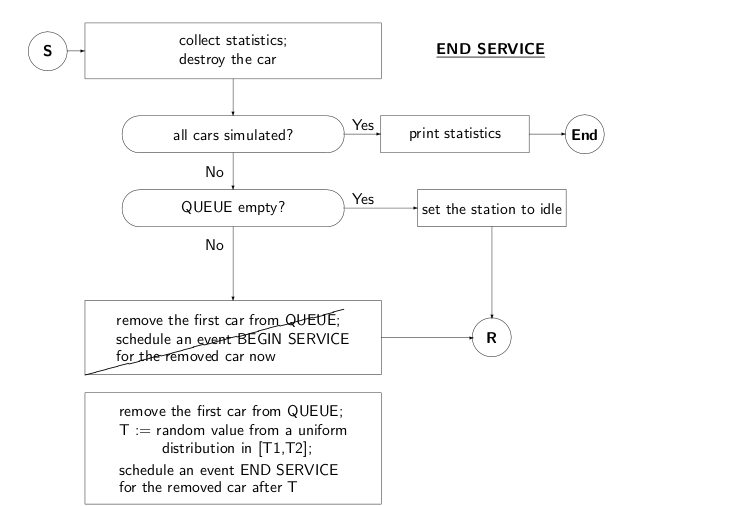
\includegraphics[width=\textwidth]{images/cap11fig12.png}
  \label{cap11fig12}
  \caption{Il nuovo evento {\em fine servizio}}
\end{figure}

Quindi si estrarre la prima auto in coda, e invece di innescare
immediatamente l'evento ``inizio servizio'', si calcola un ritardo $T$
random e si innesca direttamente l'evento ``fine servizio'' dopo un
ritardo pari a $T$. In questo modo abbiamo 2 eventi anzich\'e 3.

\par\bigskip

Facciamo ora un esempio un po pi\`u complesso. Simuliamo un piccolo
ospedale diviso in due reparti: il reparto per i malati gravi, e il
reparto per i malati non gravi. Assumiamo che i pazienti arrivino
secondo una distribuzione di Poisson di valor medio $\lambda$, e che
un paziente che arriva \`e {\bf grave} con probabilit\`a {\bf PG},
{\bf normale} con probabilit\`a {\bf 1-PG}. Sia {\bf NLG} il numero di
letti disponibili nel reparto dei malati gravi, ed {\bf NLN} il numero
di letti disponibili nel reparto dei malati normali. Se un paziente
grave arriva e non ci sono posti nel suo reparto, dato che \`e inutile
sistemarlo nel reparto dei malati normali (non essendoci l\`i
l'apparecchiatura necessaria), viene respinto e si considera uscito
dal sistema. Se invece arriva un paziente non grave e non ci sono
posti nol suo reparto, verr\`a messo in attesa. La degenza dei
pazienti gravi ha durata uniforme in $[DMIG,DMAG]$: al termine della
cura il paziente sopravvive con probabilit\`a {\bf PS} e passa al
reparto dei pazienti normali, oppure decede con probabilit\`a {\bf
  1-PS} ed in tal caso esce dal sistema. Per i pazienti normali invece
la durata della cura \`e uniforme in $[DMIN,DMAN]$. Si vogliono
simulare completamente $NTOT$ pazienti.

\begin{figure}[H]
  \centering
  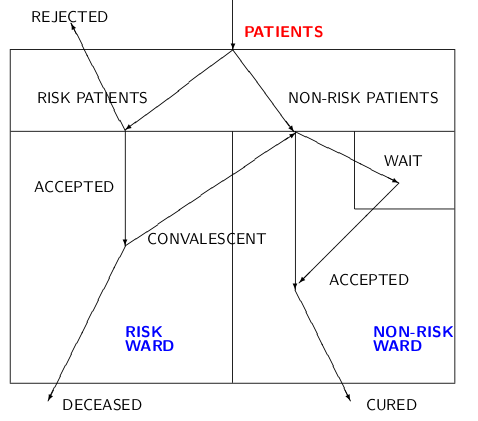
\includegraphics[width=0.6\textwidth]{images/cap11fig13.png}
\end{figure}


Anche in questo caso mostriamo, attraverso un diagramma temporale, una
possibile evoluzione del sistema al fine di evidenziare gli eventi
possibili. A tal scopo poniamo $NLG=NLN=1$ ed usiamo due assi
temporali distinti per i due reparti. Indichiamo con $A_i$ l'arrivo
del paziente i-esimo (grave o normale); con $IDG_i$ e $FDG_i$ l'inizio
e la fine della degenza del paziente grave i-esimo nel reparto dei
malati gravi; con $IDN_i$ e $FDN_i$ l'inizio e la fine della degenza
del paziente (grave, se viene dal reparto dei malati gravi, o normale)
i-esimo nel reparto per pazienti normali. Ecco una possibile sequenza
di eventi.

\begin{figure}[H]
  \centering
  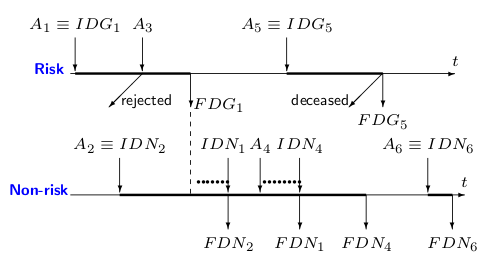
\includegraphics[width=0.8\textwidth]{images/cap11fig14.png}
\end{figure}

Seguendo l'evoluzione del paziente 1, vediamo che arriva nell'istante
$A_1$, e inizia la cura perch\'e il reparto \`e libero, termina la cura
($FDG_1$) e si mette in coda per entrare nel reparto per pazienti
normali (perch\'e questo nel frattempo si \`e occupato); inizia la
degenza in tale reparto ($IDN_1$) e poi termina ($FDN_1$) e il
paziente esce dal sistema.

Ecco il possibile diagramma degli inneschi:

\begin{figure}[H]
  \centering
  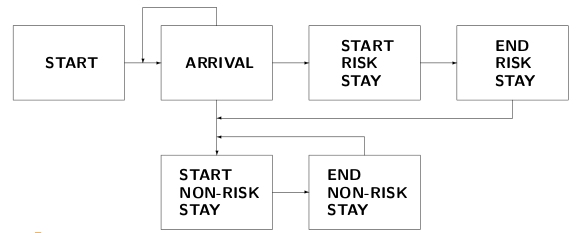
\includegraphics[width=0.8\textwidth]{images/cap11fig15.png}
\end{figure}

Anche in questo caso possiamo eliminare degli eventi: ogni volta che
vediamo che c'\`e l'inizio e la fine di un evento, deve venirci il
sospetto che l'inizio dell'evento coincida con uno o pi\`u eventi. In
questo esempio l'evento ``inizio degenza grave'' coincide sempre con
un arrivo: allora possiamo modificare il modello, facendo in modo che
quando arriva un paziente grave, se ci sono posti liberi nel reparto,
non si innesca l'evento ``inizio degenza grave'', ma direttamente
l'evento ``fine degenza grave'' dopo un ritardo $T$ random.

Inoltre l'evento ``inizio degenza normale'' coincide sempre con un
``arrivo'' o con un ``fine degenza grave'' o ancora con un ``fine
degenza normale'': quindi a partire da questi tre eventi, invece di
innescare l'evento ``inizio degenza normale'' inneschiamo direttamente
``fine degenza normale'' con un ritardo random $T$.

Ecco dunque lo schema a blocchi semplificato:

\begin{figure}[H]
  \centering
  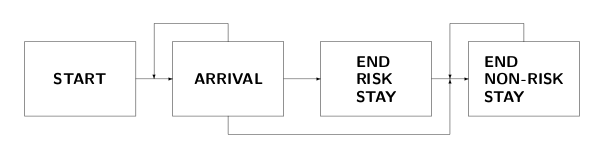
\includegraphics[width=0.9\textwidth]{images/cap11fig16.png}
\end{figure}

Vediamo ora i diagrammi di flusso.

L'evento iniziale ``start'' \`e semplicissimo: semplicemente legge i
parametri, inizializza lo stato del sistema ed innesca immediatamente
il primo arrivo.

\begin{figure}[H]
  \centering
  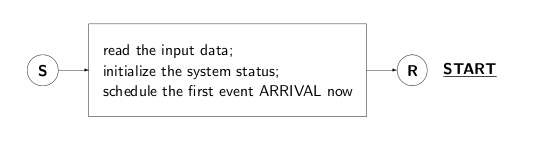
\includegraphics[width=0.75\textwidth]{images/cap11fig17.png}
\end{figure}

Nell'evento ``arrivo'', si genera il ritardo casuale $T$ con cui innescare
l'arrivo successivo, poi si vede se il paziente \`e grave o no. Se \`e
grave e non ci sono letti liberi, il paziente deve uscire, quindi
vengono raccolte le statistiche e viene distrutto il paziente. Inoltre
se \`e l'ultimo paziente da simulare si stampano le statistiche e
termina la simulazione, altrimenti il paziente esce ma la simulazione
continua. Se il paziente \`e grave e c'\`e posto nel reparto, si
incrementa il numero di letti occupati, si genera un valore casuale
$T$ con distribuzione uniforme in $[DMIG,DMAG]$, e si innesca l'evento
``fine degenza'' con ritardo $T$. Se il paziente \`e normale, viene
eseguito il sottoprogramma (che non \`e un evento) ``degenza
normale''. \`E nella pratica una chiamata a procedura: una volta
terminato il sottoprogramma, si torna nell'evento ``arrivo'' e si
esce.

\begin{figure}[H]
  \centering
  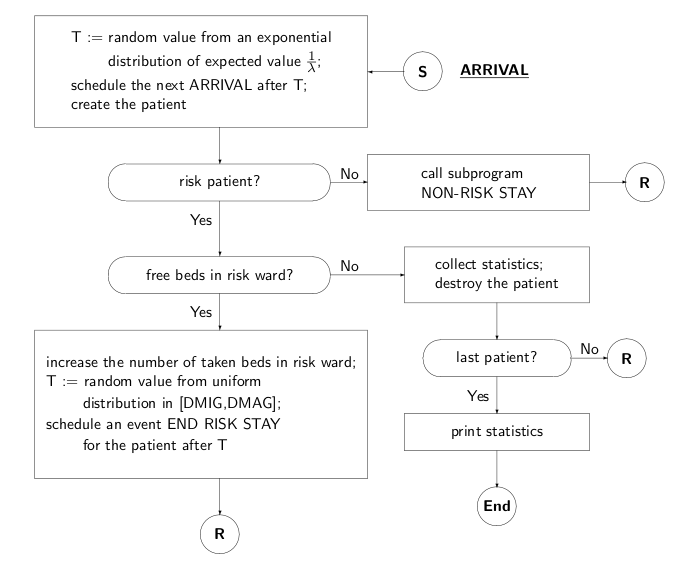
\includegraphics[width=0.9\textwidth]{images/cap11fig18.png}
\end{figure}

Il sottoprogramma ``degenza normale'' pu\`o essere rappresentato
mediante il seguente diaframma di flusso:

\begin{figure}[H]
  \centering
  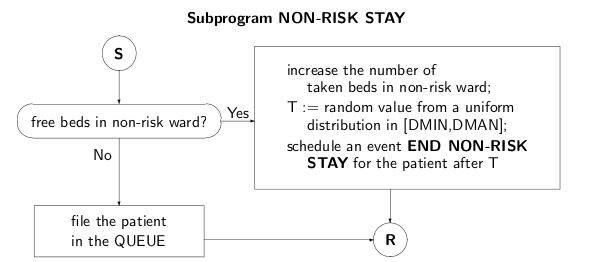
\includegraphics[width=0.85\textwidth]{images/cap11fig19.png}
\end{figure}

In pratica vede se ci sono letti liberi nel reparto: se ci sono,
incrementa il numero di letti occupati, calcola un valore casuale $T$
con distribuzione uniforme in $[DMIN,DMAN]$ ed innesca un evento
``fine degenza normale'' con ritardo $T$; se invece non ci sono letti
liberi, il paziente viene inserito nell'insieme CODA. In entrabi i
casi poi si esce dal sottoprogramma tornando all'evento chiamante (che
in questo caso \`e ``arrivo'').

Quindi i linguaggi di simulazione possono prevedere normali
sottoprogrammi: il sottoprogramma appena scritto viene chiamato non
solo dall'evento ``arrivo'' ma anche dall'evento ``fine degenza
normale''. Perci\`o si \`e preferito scriverlo come sottoprogramma
anzich\'e riscriverlo in due punti diversi (il che sarebbe stato
equivalente). 

Vediamo ora l'evento ``fine degenza grave'':

\begin{figure}[H]
  \centering
  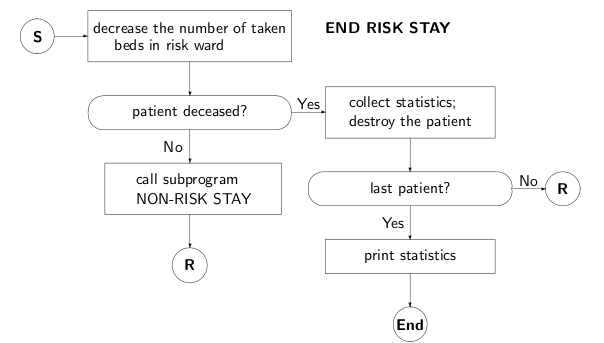
\includegraphics[width=0.85\textwidth]{images/cap11fig20.png}
\end{figure}

Si decrementa prima di tutto il numero di letti occupati nel reparto,
e poi si controlla se il pazionte \`e morto o no: se \`e morto si
raccolgono le statistiche e si esce dall'evento (anche in questo caso
si controlla se \`e l'ultimo paziente simulato, e in caso affermativo
la simulazione termina dopo aver stampato le statistiche); se non \`e
morto si esegue il sottoprogramma ``degenza normale'' e poi si esce
dall'evento.

Infine vediamo l'evento ``fine degenza normale'':

\begin{figure}[H]
  \centering
  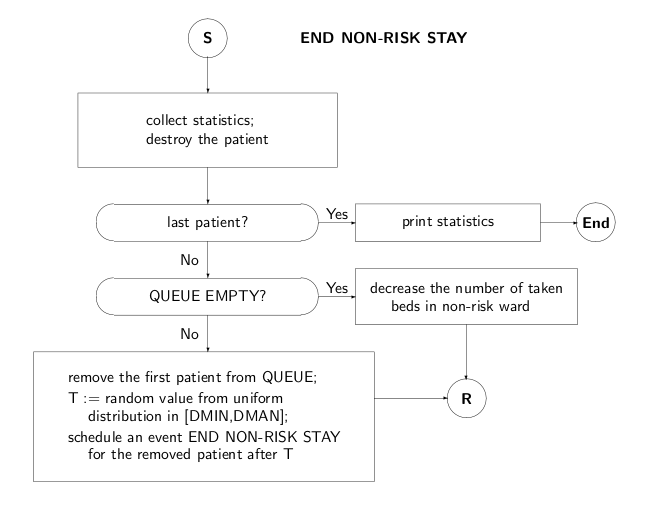
\includegraphics[width=\textwidth]{images/cap11fig21.png}
\end{figure}

Prima di tutto si raccolgono le statistiche e si distrugge il paziente
(cio\`e si libera l'area di memoria). Se \`e l'ultimo paziente della
simulazione si stampano le statistiche e la simulazione
termina. Altrimenti si controlla la coda dei pazienti: se \`e vuota si
decrementa il numero di letti occupati nel reparto e si esce
dall'evento; se non \`e vuota si estrae il primo paziente, si calcola
un valore random $T$ con distribuzione uniforme in $[DMIN,DMAN]$ e si
innesca un evento ``fine degenza normale'' con ritardo $T$.

Anche la parte del programma che controlla se si \`e alla fine della
simulazione e stampa eventualmente le statistiche potrebbe essere
scritta come sottoprogramma, dato che \`e richiamata pi\`u volte da
eventi diversi.

\section{Le componenti della simulazione}
Le componenti fondamentali di un modello di simulazione sono le {\bf
  entit\`a} e gli {\bf eventi}. 

Le {\bf entit\`a} sono gli oggetti creati dal modello e si classificano
in:

\begin{itemize}
\item Entit\`a {\bf temporanee}, che sono le entit\`a che vengono create
  quando entrano nel sistema e distrutte quando ne escono, quindi
  restano nel sistema per un tempo limitato. Degli esempi sono {\em
    auto} e {\em paziente}. Queste entit\`a possono avere degli
  attributi che vengono chiamati {\bf attributi temporanei} (ad
  esempio l'istante di ingresso in coda, il tipo di malattia, ecc.).
\item Entit\`a {\bf permanenti}, che sono le entit\`a che sono sempre
  presenti durante tutta la simulazione. L'entit\`a permanente
  fondamentale \`e il {\bf sistema} stesso (ad esempio la stazione di
  servizio, l'ospedale). Quest'entit\`a non viene definita in modo
  esplicito, e possiede gli {\bf attributi permanenti} (ad esempio
  quelli riguardanti lo stato del sistema, come {\em stazione libera o
    occupata}, e i dati di input, come {\em numero letti} e i dati
  riguardanti le distribuzioni di probabilit\`a). Poi ci sono le altre entit\`a
  permanenti, quelle vere e proprie, che noi non abbiamo ancora visto
  negli esempi, e che sono rappresentate tramite {\bf indici}.
\end{itemize}

Gli {\bf eventi} sono i sottoprogrammi che contengono le istruzioni da
eseguire quando cambia lo stato del sistema. Essi determinano gli
eventi futuri e li innescano. Quando termina un evento, il sistema
manda in esecuzione l'evento innescato per l'istante futuro pi\`u
prossimo ed aggiorna il tempo simulato. Possiamo distinguere:

\begin{itemize}
\item Eventi {\bf interni} o {\bf endogeni}: sono quelli innescati da
  altri eventi (tutti quelli visti fin ora, {\em Arrivo, Fine
    servizio, Fine Degenza}, tranne {\em Start}).
\item Eventi {\bf esterni} o {\bf esogeni}: sono quelli innescati
  dall'esterno (come appunto l'evento {\em Start}). 
\end{itemize}

Negli esempi visti fin ora era richiesto di far terminare la
simulazione dopo aver simulato {\em completamente} un certo numero di
entit\`a. Per evitare che venissero considerate nelle statistiche anche
le entit\`a non completamente simulate (ad esempio quelle ancora in
coda), la raccolta dei dati statistici \`e stata fatta solo nel momento
in cui l'entit\`a stava per uscire dal sistema. 

Vediamo ora un ultimo esempio prima di passare a parlare dei {\em
  linguaggi di simulazione}.

Simuliamo la versione semplificata dell'unit\`a multidisco
schematizzata in figura:

\begin{figure}[H]
  \centering
  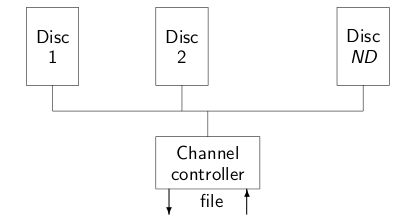
\includegraphics[width=0.6\textwidth]{images/cap11fig22.png}
\end{figure}

I dischi sono numerati da $1$ a $ND$, e ogni disco ha $NC$ cilindri
anch'essi numerati da $1$ a $NC$. I file devono essere letti o scritti
da/in un determinato cilindro di un certo disco.

I file da memorizzare o leggere (\`e indifferente) arrivano secondo una
distribuzione di Poisson di valor medio $\lambda$. Ogni file ha una
{\em lunghezza} $L$ distribuita uniformemente in $[MIN,MAX]$, e
richiede un disco di competenza distribuito uniformemente in $[1,ND]$
e un cilindro distribuito uniformemente in $[1,NC]$.

Se il disco richiesto non \`e libero, il file attende in una coda
associata al disco richiesto. In tale coda hanno la precedenza i file
con tempo di trasmissione minore.

Se invece il disco \`e libero avviene il posizionamento della testina
in corrispondenza del cilindro richiesto: il posizionamento della
testina richiede un tempo dato da una funzione nota $f_1(D)$ della
distanza $D$ tra la posizione attuale della testina e la nuova
posizione richiesta. 

\begin{figure}[H]
  \centering
  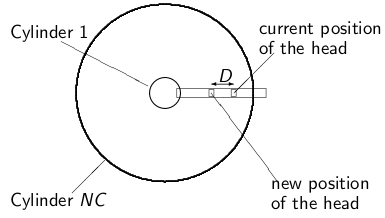
\includegraphics[width=0.5\textwidth]{images/cap11fig23.png}
\end{figure}

Terminato il posizionamento, se il canale \`e libero si attende la
rotazione del disco, distribuita uniformemente in $[0,TR]$, e quindi
la trasmissione, il cui tempo \`e dato da una funzione della lunghezza
$L$ del file, $f_2(L)$.

Se invece il canale \`e occupato, il file attende in una coda nella
quale hanno precedenza i file relativi a dischi con numero d'ordine
minore. 

\`E richiesto di terminare la simulazione dopo $TS$ unit\`a di tempo.

In questo esempio le {\bf entit\`a permanenti} sono il sistema (con
attributi permanenti $\lambda, ND, NC, TR, f1, f2$ e lo stato del
canale), e i dischi, rappresentati da interi tra $1$ e $ND$, (che
hanno come attributi lo stato del disco e la posizione corrente della
testina). Le {\bf entit\`a temporanee} invece sono i file (che hanno
come attributi la lunghezza, il disco richiesto e il cilindro
richiesto).

Vediamo un diagramma temporale d'esempio, per vedere i vari eventi che
possono avvenire. Per semplicit\`a consideriamo la presenza di soli due
dischi. Avremo tre assi temporali: due per i dischi e uno per il
controllore di canale.

\begin{figure}[H]
  \centering
  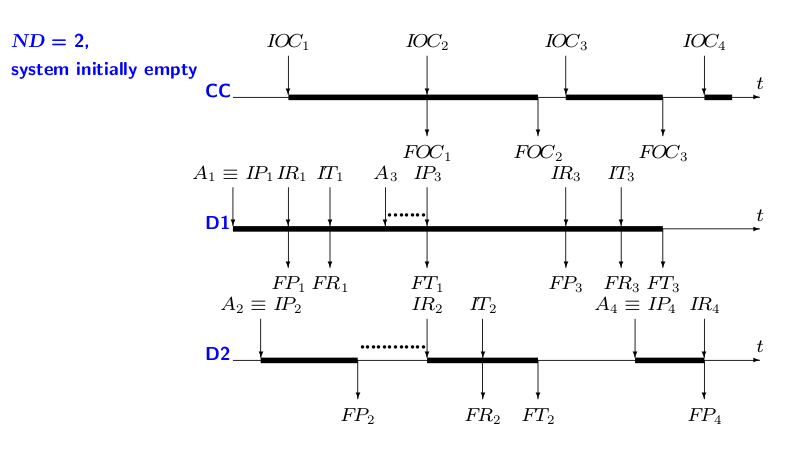
\includegraphics[width=\textwidth]{images/cap11fig24.png}
\end{figure}

Nell'istante A1 arriva un file per il disco 1, il disco \`e libero
quindi nello stesso istante inizia il posizionamento della testina per
questo file ($IP_1$). Termina il posizionamento ($FP_1$) e dato che il
controllore del canale \`e libero inizia la rotazione e l'occupazione
del canale ($IR_1$ e $IOC_1$). Poi finisce la rotazione ($FT_1$) e
nello stesso istante inizia la trasmissione $IT_1$ per poi terminare
($FT_1$). Questa \`e l'evoluzione del file numero 1. Nel frattempo
vediamo che arriva il file 2 per il disco 2 e trova il disco libero
quindi inizia il posizionamento. Quando termina il posizionamento
per\`o il controllore \`e ancora occupato per il file 1 quindi il file 2
si accoda. Quando finisce l'occupazione del canale da parte del primo
file, inizia l'occupazione del canale da parte del secondo file ed
inizia la rotazione. Finisce la rotazione, inizia la trasmissione, e
poi termina ($FT_2$) e si libera quindi il canale. Non ci sono altri
file in coda quindi il canale resta libero per un p\`o. E cos\`i via...

Ecco il diagramma a blocchi degli innesti:

\begin{figure}[H]
  \centering
  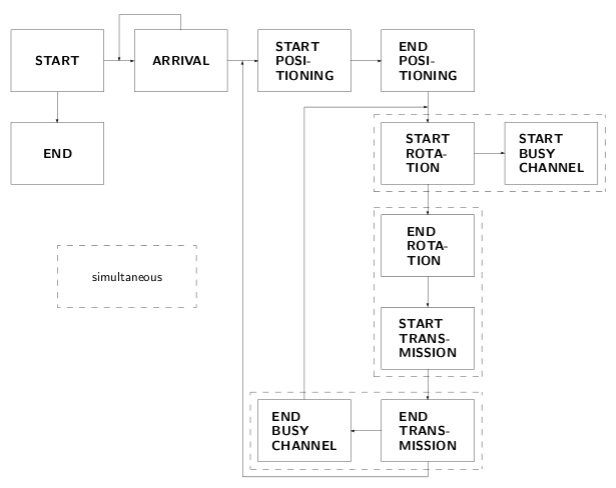
\includegraphics[width=\textwidth]{images/cap11fig25.png}
\end{figure}

Questo contiene tutti gli eventi, ma notiamo che pu\`o essere ridotto
molto in quanto alcuni eventi coincidono sempre temporalmente. In
particolare gli eventi racchiusi dalle linee tratteggiate: quando
inizia la rotazione inizia sempre l'occupazione del canale, quando
finisce la rotazione inizia sempre la trasmissione, quando finisce la
trasmissione finisce sempre l'occupazione del canale. Ecco dunque lo
schema semplificato un p\`o:

\begin{figure}[H]
  \centering
  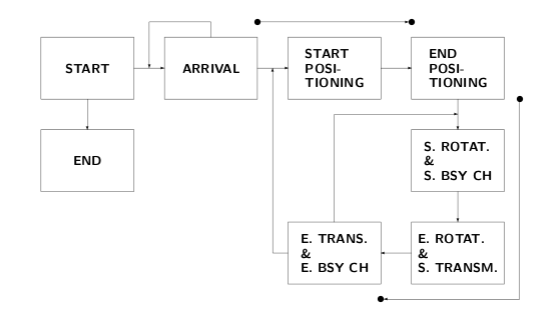
\includegraphics[width=\textwidth]{images/cap11fig26.png}
\end{figure}

Ancora vediamo che ci sono degli eventi che possono essere eliminati:
possiamo compattare in un unico evento alcuni gruppi di eventi. In
particolare possiamo far collassare i due eventi ``inizio
posizionamento'' e ``fine posizionamento'' in un unico evento ``fine
posizionamento'' cos\`i se il disco \`e libero (nell'evento ``arrivo'')
si innesca direttamente l'evento ``fine posizionamento'' dopo un certo
ritardo opportunamente calcolato (come vedremo). E i tre eventi in
basso a destra possono essere compattati in un unico evento ``fine
occupazione canale'', cio\`e se il canale \`e libero (al momento della
fine del posizionamento) si innesca direttamente la fine
dell'occupazione del canale dopo un ritardo opportunamente
calcolato. Ecco dunque lo schema a blocchi definitivo:

\begin{figure}[H]
  \centering
  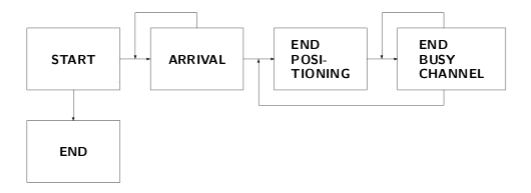
\includegraphics[width=\textwidth]{images/cap11fig27.png}
\end{figure}

Notiamo inoltre gli eventi esterni ``start'' e ``end'': l'evento
``start'' oltre ad innescare il primo arrivo, innesca anche la fine
della simulazione dopo un tempo pari a $TS$.

Vediamo ora i diagrammi di flusso degli eventi del sistema.

Iniziamo dai due pi\`u semplici: {\em inizio} e {\em fine}.

Nell'evento {\em inizio} si leggono i parametri di input, si
inizializza lo stato del sistema, e inoltre si innesca l'arrivo del
primo file subito e la fine della simulazione dopo un tempo $TS$ che
\`e il tempo di simulazione prefissato.

\begin{figure}[H]
  \centering
  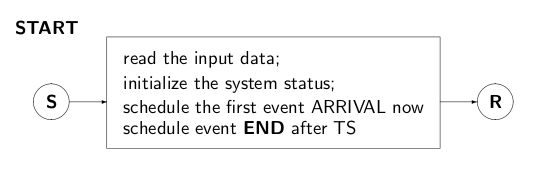
\includegraphics[width=0.7\textwidth]{images/cap11fig28_1.png}
\end{figure}

Nell'evento {\em fine} invece si stampano semplicemente le
statistiche.

\begin{figure}[H]
  \centering
  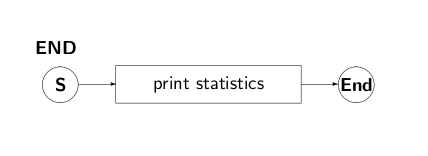
\includegraphics[width=0.7\textwidth]{images/cap11fig28_2.png}
\end{figure}

Passiamo agli eventi pi\`u interessanti: gli eventi interni.

Nell'evento {\em arrivo} come prima cosa viene calcolato un valore
casuale $T$ con distribuzione esponenziale di valor medio $1/\lambda$;
poi si innesca il prossimo arrivo con ritardo $T$, si genera il file e
se ne determinano casualmente la lunghezza $L$ e il disco e il
cilindro richiesti. Se il disco \`e libero viene occupato, viene
calcolata la distanza $D$, e innescato l'evento ``fine
posizionamento'' per il file con ritardo $f_1(D)$. Se il disco non \`e
libero si accoda il file nella coda associata al disco. In entrambi i
casi l'evento ``arrivo'' si conclude.

\begin{figure}[H]
  \centering
  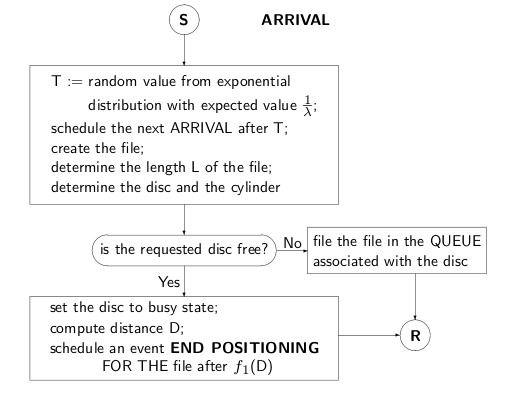
\includegraphics[width=0.9\textwidth]{images/cap11fig29.png}
\end{figure}

Passiamo all'evento ``fine posizionamento''. Se il controllore di
canale \`e libero si occupa il canale, viene calcolato un valore
casuale $T$ con distribuzione uniforme in $[0,TR]$ e si innesca
l'evento ``fine occupazione canale'' per il file, con ritardo
$T+f_2(L)$ dove $T$ \`e il tempo di rotazione e $f_2(L)$ \`e il tempo
necessario a trasmettere il file. Se il controllore di canale \`e
occupato si mette il file nella coda associata al controllore. Infine
termina l'evento.

\begin{figure}[H]
  \centering
  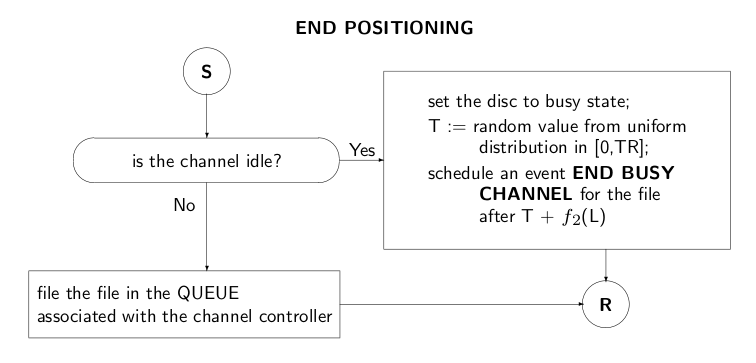
\includegraphics[width=\textwidth]{images/cap11fig30.png}
\end{figure}

Nell'evento ``fine occupazione canale'' si raccolgono le statistiche e
si distrugge il file. Poi se la coda del disco richiesto \`e vuota si
libera il disco; mentre se non \`e vuota si estrae il primo file dalla
coda associata a tale disco, si calcola la distanza $D$ e si innesca
un evento ``fine posizionamento'' per il file estratto, con ritardo
$f_1(D)$. In estrambi i casi, dopo si controlla la coda del la coda
del controllore di canale: se \`e vuota si libera il canale e termina
l'evento, mentre se non \`e vuota si estrae il primo file in coda, si
calcola un valore random $T$ con distribuzione uniforme in $[0,TR]$,
si innesca un evento ``fine occupazione canale'' per il file estratto
con ritardo $T+f_2(L)$, e termina l'evento.

\begin{figure}[H]
  \centering
  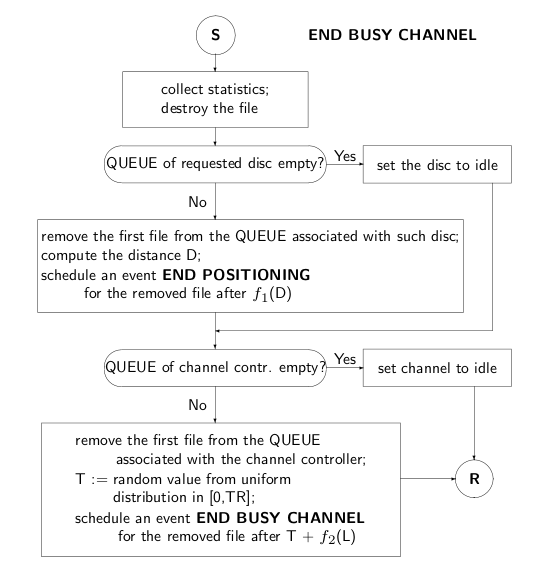
\includegraphics[width=0.9\textwidth]{images/cap11fig31.png}
\end{figure}

\section{Linguaggi di simulazione}
Esistono due famiglie distinte di modelli di simulazione: {\em
  discreti e continui}. Nell'ambito della simulazione discreta (che \`e
quella che ci interessa) esistono due principali approcci e due
relative famiglie di linguaggi. L'approccio che abbiamo usato noi \`e
detto {\bf programmazione degli eventi} o {\bf schedulazione degli
  eventi}, e ormai sappiamo bene come funziona. L'altro approccio \`e
noto come {\bf interazione dei processi}: in questo approccio, gli
eventi che descrivono le varie fasi della vita di un'entit\`a sono fusi
in un unico diagramma di flusso, il {\bf processo}. Quindi un processo
coincide con l'entit\`a, \`e una sequenza cronologica di eventi. Ad
esempio nell'esempio della stazione di servizio si avrebbe, secondo
tale approccio, un unico processo {\bf auto} dato dalla concatenazione
dei due eventi {\em arrivo} e {\em fine servizio}. Per simulare
l'evoluzione nel tempo si usano istruzioni del tipo ``aspetta fino
a..'', ``riattiva il processo'', ecc. A livello didattico si
preferisce il primo approccio perch\'e tradurre i modelli ottenuti
secondo questo approccio, in modelli equivalenti basati sul secondo
approccio \`e pi\`u semplice della traduzione opposta. Inoltre se non si
pu\`o o non si vuole usare un linguaggio di simulazione, un modello
basato sul primo approccio \`e pi\`u semplice da implementare con un
linguaggio general purpose.

I principali linguaggi di simulazione sono di tipo imperativo. Tra
questi abbiamo:

\begin{itemize} 
\item {\bf Simula I} e {\bf Simula 67}: oggi raramente utilizzati,
  seguono l'approccio dell'interazione dei processi, hanno introdotto
  i concetti di oggetti e classi e hanno fortemente influenzato il
  C++.
\item {\bf Simscript I} e {\bf Simscript II.5}: seguono l'approccio
  della schedulazione degli eventi. Simscript \`e il linguaggio di
  simulazione pi\`u potente e usato, e ha influenzato Simula anche se
  rispetto ad esso \`e pi\`u semplice da usare e pi\`u efficiente.  Per
  spiegare i prossimi concetti utilizzeremo Simscript II.5. Questo
  linguaggio possiede anche le istruzioni per realizzare l'altro
  approccio (interazione dei processi): chiaramente per\`o non possono
  essere usati entrambi gli approcci contemporaneamente.
\end{itemize}

Esistono anche linguaggi di simulazione di tipo interattivo, come {\bf
  Arena} (che segue l'approccio dell'interazione dei processi), e {\bf
  SAS/OR} (che segue l'approccio della schedulazione degli eventi):
sono entrabi semplici da usare ma meno potenti.

Infine possiamo implementare la simulazione con linguaggi general
purpose (ad esempio Java), ma con molta pi\`u difficolt\`a.

\subsection{Istruzioni tipiche della simulazione}
Per descrivere le principali istruzioni relative alla simulazione
faremo riferimento al linguaggio SIMSCRIPT II.5, ma le istruzioni che
vedremo sono concettualmente analoghe a quelle degli altri linguaggi.

\subsubsection{Entit\`a temporanee}
L'istruzione di {\bf creazione} \`e questa:

\begin{verbatim}
CREATE [A,AN,THE] en [CALLED p]
\end{verbatim}

Con questa istruzione viene riservata un'area di memoria per una nuova
entit\`a della classe {\em en}, e si definisce una variabile locale
(locale all'evento in cui ci troviamo) di nome {\em p} contenente il
puntatore all'area di memoria: se {\em CALLED p} \`e omesso, tale
variabile ha nome {\em en}. Per creare una sola entit\`a si preferisce
la forma breve {\em CREATE AUTO}, altrimenti \`e necessaria la forma
lunga per poterle poi distinguere, ad esempio:

\begin{verbatim}
CREATE A CAR CALLED A1 
CREATE A CAR CALLED A2
\end{verbatim}

L'istruzione di {\bf distruzione} \`e questa:

\begin{verbatim}
DESTROY THE en [CALLED p]
\end{verbatim}

Con questa istruzione si rilascia l'area di memoria della classe {\em
  en} avente per puntatore {\em p} (o {\em en} se {\em CALLED p} \`e
omesso).

Tali entit\`a temporanee possono avere degli attributi temporanei, che
hanno la seguente forma:

\begin{verbatim}
attributo(p)
\end{verbatim}

dove {\em p} \`e il puntatore all'entit\`a temporanea a cui l'attributo
si riferisce. Ad esempio con le istruzioni

\begin{verbatim}
CREATE A CAR CALLED A1
LET TYPE(A1) = X
\end{verbatim}

abbiamo creato un'entit\`a {\em A1} della classe {\em CAR} e abbiamo
posto il tipo di {\em A1} ad {\em X}. Tale informazione viene messa
nell'area di memoria riservata all'entit\`a creata. 

Consideriamo l'esempio della stazione di servizio, e supponiamo che
ogni entit\`a AUTO abbia due attributi, {\em TIS} (istante di ingresso
nel sistema), e {\em TIPO} (X o Y). Vediamo che effetto ha nella
memoria la seguente sequenza di eventi:

\begin{figure}[H]
  \centering
  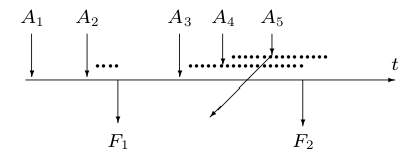
\includegraphics[width=0.6\textwidth]{images/cap11fig32.png}
\end{figure}

dove $A_i$ rappresenta l'arrivo dell'auto i-esima nel sistema, ed
$FS_i$ indica l'evento fine servizio dell'auto i-esima.

\begin{figure}[H]
  \centering
  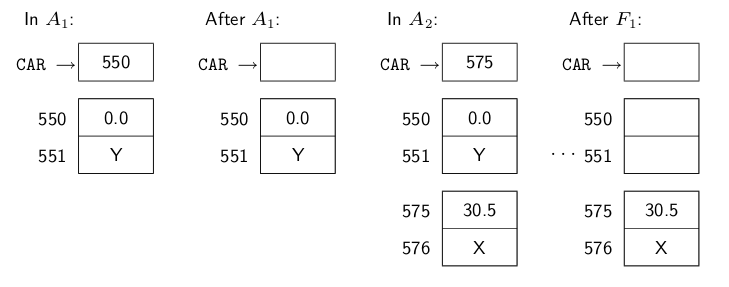
\includegraphics[width=0.9\textwidth]{images/cap11fig33.png}
\end{figure}

\subsubsection{Entit\`a permanenti}
Abbiamo detto che la principale entit\`a permanente, che non manca mai,
\`e il sistema stesso. Questo pu\`o avere {\bf attributi permanenti} che
sono variabili globali, come ad esempio il numero di letti
disponibili, il numero di utenti da simulare, i parametri delle
distribuzioni con con cui succedono i vari eventi. Inoltre il sistema
pu\`o avere delle code senza indice (come la coda d'attesa per i
pazienti normali). Il sistema \`e creato automaticamente e non viene
mai distrutto.

Poi abbiamo le entita permanenti vere e proprie, come ad esempio i
dischi di uno degli esempi precedenti. Anche queste possono avere
degli attributi permanenti (variabili globali). Tali attributi sono
rappresentate da variabili con indice, il cui indice rappresenta
un'entit\`a permanente, ad esempio scrivendo {\em STATO(j)} stiamo ad
indicare lo stato (libero o occupato) del disco {\em j}. Le entit\`a
permanenti possono avere associate anche delle code con indice: {\em
  CODA(j)=coda associata al disco j}.

Le intit\`a permanenti si creano tutte insieme mediante le istruzioni:

\begin{verbatim}
READ N.en
CREATE EVERY en
\end{verbatim}

cio\`e prima si definisce il numero di entit\`a della classe {\em en} da
creare, e poi si creano.

\subsubsection{Insiemi}
Gli insiemi sono le code che abbiamo visto fin ora negli esempi. Gli
insiemi sono caratterizzati da:
\begin{itemize}
\item {\bf membri}, che sono in genere entit\`a temporanee; 
\item {\bf proprietari}, che sono entit\`a permanenti (il sistema
  stesso, per gli insiemi senza indice, le entit\`a permanenti vere e
  proprie, per gli insiemi con indice);
\item {\bf modalit\`a di ordinamento}: FIFO, LIFO, {\bf ranked} (in cui
  la precedenza \`e data dal valore crescente o decrescente di un
  attributo delle entit\`a membre).
\end{itemize}

Vediamo le principali istruzioni con gli insiemi:

\begin{verbatim}
FILE THE p IN THE s
\end{verbatim}

inserisce l'entit\`a puntata da {\em p} nell'insieme {\em s}.

\begin{verbatim}
REMOVE THE FIRST q FROM THE s
\end{verbatim}

estrae il primo elemento dall'insieme {\em s} e memorizza il suo
puntatore nella variabile locale {\em q}.  

\begin{verbatim}
REMOVE THE p FROM THE s 
\end{verbatim}

rimuove l'entit\`a puntata da {\em p} dall'insieme {\em s}.

\begin{verbatim}
IF THE s IS EMPTY I 
IF THE s IS NOT EMPTY I 
\end{verbatim}

la prima esegue l'istruzione {\em I} se {\em s} \`e vuoto, la seconda
la esegue se l'insieme non \`e vuoto.

\subsubsection{Eventi ed event notice}
Gli {\bf eventi esterni} vengono innescati mediante dati di ingresso e
non richiedono di riservare o distruggere aree di memoria. Invece gli
{\bf eventi interni} vengono innescati da altri eventi, e richiedono
un certo numero di dati (come ad esempio l'istante in cui devono
avvenire, l'entit\`a temporanea a cui si riferiscono, ecc.), quindi per
tali eventi c'\`e bisogno di un'area di memoria associata. Perci\`o ad
ogni evento \`e automaticamente associata una particolare entit\`a
temporanea avente il suo stesso nome, detta {\bf event notice}. Gli
event notice devono essere creati nel momento in cui viene innescato
l'evento relativi, e devono essere distrutti appena l'evento si
verifica. Essi possono possedere attributi che tipicamente vengono
utilizzati per trasmettere i puntatori alle entit\`a a cui si
riferiscono. Al momento dell'esecuzione di un evento, il puntatore al
suo event notice viene salvato automaticamente in una variabile locale
avente il nome dell'evento.

Chiariamo il tutto con il solito esempio della stazione di servizio.
Assumiamo che CAR contenga il puntatore all'auto appena creata, dunque
il blocco da eseguire quando l'auto occupa la stazione \`e questo:

\begin{figure}[H]
  \centering
  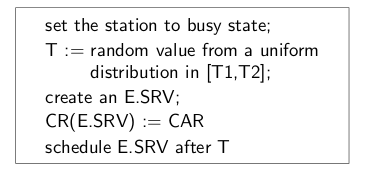
\includegraphics[width=0.6\textwidth]{images/cap11fig34.png}
\end{figure}

Cio\`e occupa la stazione, genera un ritardo, crea l'evento fine
servizio (E.SRV), e genera quindi l'event notice E.SRV, dopodich\'e
crea un attributo CR per questo event notice e gli assegna il
puntatore all'auto a cui l'evento si riferisce. Infine innesca E.SRV
con il ritardo generato precedentemente.

Nell'evento di fine servizio, se l'evento va re-innescato, \`e
possibile sia distruggere l'event notice e crearne uno nuovo, sia
ritardare la distruzione dell'event notice ed eventualmente
re-innescare lo stesso. La seconda soluzione \`e pi\`u efficiente ed \`e
mostrata di seguito:

\begin{figure}[H]
  \centering
  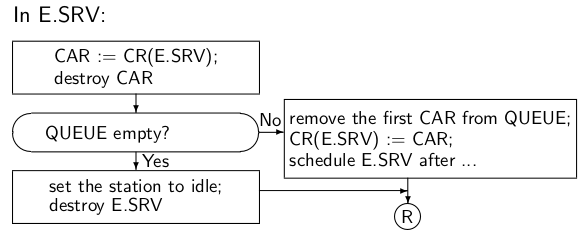
\includegraphics[width=0.9\textwidth]{images/cap11fig35.png}
\end{figure}

Si recupera il puntatore all'auto, si distrugge l'entit\`a. Se la coda
\`e vuota si libera la stazione e si distrugge l'event-notice (o
l'evento?), mentre se non \`e vuota si estrae la prima auto dalla coda,
si assegna all'attributo AUT dell'event notice il puntatore all'auto
estratta, e si re-innesca l'evento con un opportuno ritardo.

Consideriamo ancora la sequenza di eventi di prima, e vediamo cosa
succede nella memoria:

\begin{figure}[H]
  \centering
  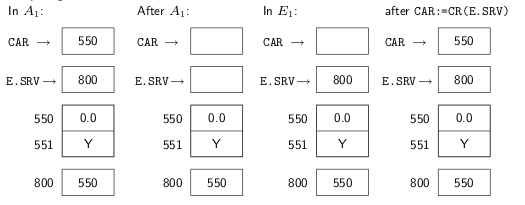
\includegraphics[width=\textwidth]{images/cap11fig36.png}
\end{figure}

L'istruzione:

\begin{verbatim}
CREATE AN ev [CALLED p] 
\end{verbatim}

riserva un'area di memoria per un nuovo event notice della classe {\em
  ev}, e definisce una variabile locale {\em p} (o {\em ev}) che
contiene il puntatore a tale area di memoria.

L'istruzione di innesco:

\begin{verbatim}
SCHEDULE THIS ev [CALLED p] AT t 
\end{verbatim}

innesca l'evento di puntatore {\em p} (o {\em ev}) per l'istante {\em
  t}. Si pu\`o fornire o l'istante di tempo assoluto di innesco, o il
ritardo rispetto all'istante attuale. A tal scopo i linguaggi
forniscono una variabile di valore pari all'istante di tempo simulato
attuale: {\bf TIME.V}. Ad esempio:

\begin{verbatim}
SCHEDULE THIS ev [CALLED p] AT TIME.V + T 
\end{verbatim}

Infine l'istruzione di disinnesco:

\begin{verbatim}
CANCEL THE ev [CALLED p] 
\end{verbatim}

disinnesca l'evento della classe {\em ev} di puntatore {\em p} (o {\em
  ev}), senza distruggere per\`o l'event notice corrispondente.

\section{Esempi avanzati di modelli di simulazione}
Vediamo ora il modello della stazione di servizio gi\`a esaminato,
dettagliando per\`o la gestione degli attributi e degli event
notice. Vogliamo determinare la percentuale di auto rifiutate e il
tempo medio trascorso in coda dalle auto servite. Si fermi la
simulazione dopo che NA auto sono uscite dal sistema. 

\begin{itemize}
\item Le entit\`a temporanee CAR hanno due attributi:
  \begin{itemize}
  \item TIC(CAR): istante di ingresso in coda;
  \item TC(CAR): tempo trascorso in coda.
  \end{itemize}
\item Il sistema ha come attributi:
  \begin{itemize}
  \item I dati di input: $\lambda$,T1,T2,NMAX,NA;
  \item I valori interni: NAS (numero di auto simulate), NAR (numero
    di auto rifiutate), TTC (tempo totale in coda), NAC (numero di
    auto in coda), STATO (= 0 se la stazione \`e libera, = 1 se la
    stazione \`e occupata).
  \end{itemize}
\item Il sistema possiede un'unica coda QUEUE (quindi il proprietario
  \`e il sistema) ad ordinamento FIFO, che ha come entit\`a membre le
  auto.
\item Gli eventi INIZIO e ARRIVO non hanno attributi;
\item L'evento E.SRV (fine servizio) ha l'attributo CR (che sta per
  car) contenente il puntatore all'entit\`a CAR interessata: quindi
  CR(E.SRV)= puntatore all'auto servita.
\end{itemize}

Vediamo dunque gli schemi a blocchi dei vari eventi.

Partiamo dall'evento INIZIO e la procedura FINE:

\begin{figure}[H]
  \centering
  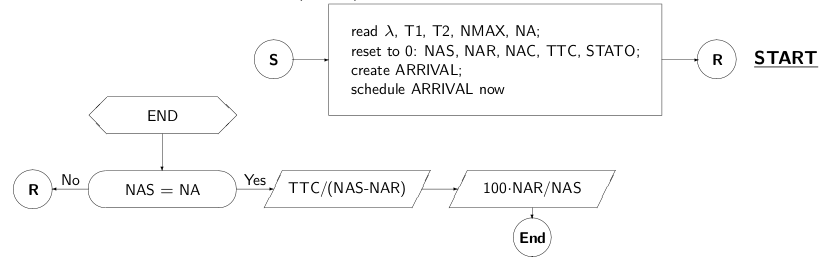
\includegraphics[width=\textwidth]{images/cap11fig37.png}
\end{figure}

Nell'evento INIZIO si leggono i parametri di ingresso, si azzerano i
valori interni, si crea e si innesca subito l'evento arrivo.

La procedura FINE invece, se abbiamo raggiunto il numero totale di
auto da simulare, si stampano le statistiche (la stampa si indica con
un parallelogramma in cui scriviamo quello che vogliamo stampare) e si
isce dalla simulazione, altrimenti si prosegue con la simulazione.

Passiamo all'evento ARRIVO:

\begin{figure}[H]
  \centering
  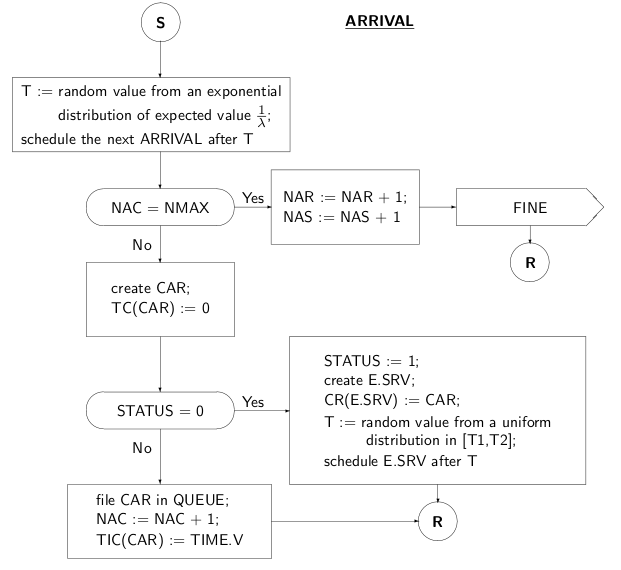
\includegraphics[width=0.9\textwidth]{images/cap11fig38.png}
\end{figure}

in cui si calcola casualmente il ritardo T e si innesca un'altro
arrivo con tale ritardo. Poi se il numero di auto in coda \`e pari al
massimo di posti in coda, si incrementa il numero di auto rifiutate e
il numero di auto simulate, e si chiama la procedura FINE; altrimenti
si crea l'entit\`a CAR e si azzera l'attributo TC di tale auto, e si va
a controllare lo STATO: se la stazione \`e libera, si occupa, si crea
l'evento di fine servizio, si crea l'attributo CR di tale evento e gli
si assegna il puntatore all'auto simulata, si genera un ritardo T e si
innesca l'evento di fine servizio con tale ritardo; se invece la
stazione \`e occupata, si inserisce l'auto in coda, si incrementa il
numero di auto in coda e si assegna l'istante di tempo attuale
all'attributo TIC dell'auto. 

Infine vediamo l'evento di fine servizio:

\begin{figure}[H]
  \centering
  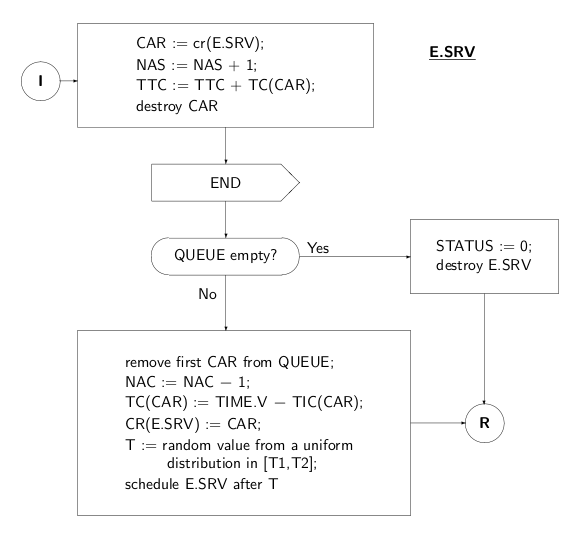
\includegraphics[width=0.9\textwidth]{images/cap11fig39.png}
\end{figure}

Si recupera prima di tutto l'auto per la quale \`e stato innescato
l'evento, si incrementa il numero di auto simulate, e si incrementa il
TTC aggiungendogli il tempo in coda dell'auto in questione. Si
distrugge poi tale entit\`a, e si chiama la procedura FINE. Se la
simulazione non \`e terminata si controlla lo stato della coda: se \`e
vuota si libera la stazione (ponendo STATO=0) e si distrugge l'evento
di fine servizio; altrimenti si estrae la prima auto dalla coda (dato
che \`e FIFO), si decrementa il numero di auto in coda, si mette
nell'attributo TC dell'auto il tempo in coda (ovvero la differenza tra
l'istante attuale e l'istante di ingresso in coda, cio\`e il TIC), si
salva il puntatore all'auto estratta nell'attributo CR dell'evento di
fine servizio, si calcola un ritardo T e si innesca (reinnesca)
l'evento di fine servizio con ritardo T.

\par\bigskip
Dunque abbiamo visto che esistono tre soli modi per la trasmissione di
informazioni tra eventi:

\begin{itemize}
\item Attributi permanenti: ad esempio TTC azzerato in INIZIO,
  aggiornato in E.SRV, e usato in FINE.
\item Attributi di event notice: ad esempio CR(E.SRV) definito in
  ARRIVO e usato in E.SRV.
\item Attributi di entit\`a temporanee inserite e rimosse da insiemi:
  ad esempio CAR inserita nella coda nell'evento ARRIVO, e rimossa in
  E.SRV dove si utilizza il TIC(CAR).
\end{itemize}

Vediamo ora l'esempio dell'ospedale: vogliamo determinare,
relativamente ad NT pazienti usciti dal sistema, il tempo medio
trascorso in coda {\bf dai pazienti che hanno dovuto attendere}, i
tempi medi trascorsi nel sistema dai pazienti gravi e dai pazienti
normali, e la percentuale dei pazienti gravi rifiutati. 

\begin{itemize}
\item Ogni entit\`a temporanea PAZIENTE ha tre attributi:
  \begin{itemize}
  \item TIS(PAZIENTE): istante di ingresso nel sistema;
  \item TIC(PAZIENTE): istante di ingresso in coda;
  \item TIPO(PAZIENTE): 1 se normale, 0 se grave.
  \end{itemize}
\item Il sistema ha come attributi:
  \begin{itemize}
  \item I dati di input: $\lambda$, NLG, NLN, PG, PS, DMIG, DMAG,
    DMIN, DMAN, NT. 
  \item I valori interni: NLOG ed NLON (numero di letti occupati nei
    due reparti), NPR, NPD, NPG (numero di pazieni gravi rifiutati,
    deceduti e guariti), NPN (numero di pazienti normali guariti), NPA
    (numero di pazienti che hanno atteso in coda), NTOT (numero di
    pazienti simulati), TTG e TTN (tempo totale trascorso nel sistema
    da pazienti gravi e normali), TTA (tempo totale trascorso dai
    pazienti in coda).
  \end{itemize}
\item Il sistema possiede un'unica coda QUEUE ad ordinamento FIFO, che
  ha come entit\`a membre i pazienti.
\item Gli eventi INIZIO e ARRIVO non hanno attributi;
\item Gli eventi E.RP e E.NRP (fine degenza graze e normale) hanno
  l'attributo PAZ (che sta per paziente) contenente il puntatore
  all'entit\`a PAZIENTE a cui sono relativi.
\end{itemize}

Vediamo dunque gli schemi a blocchi dei vari eventi.

\begin{figure}[H]
  \centering
  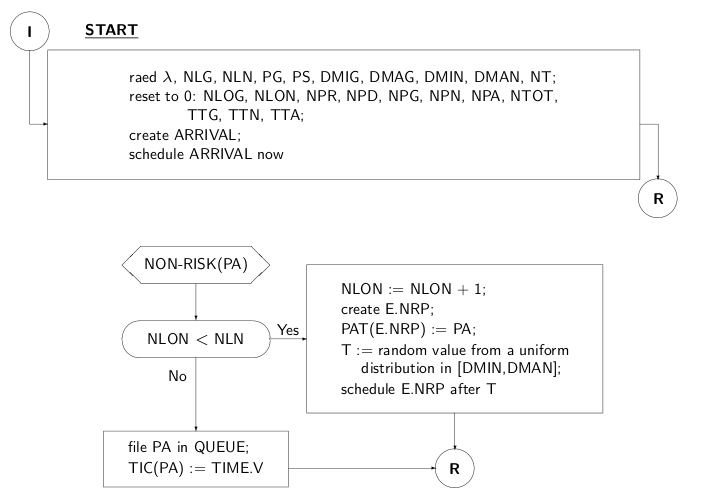
\includegraphics[width=\textwidth]{images/cap11fig40.png}
\end{figure}

\begin{figure}[H]
  \centering
  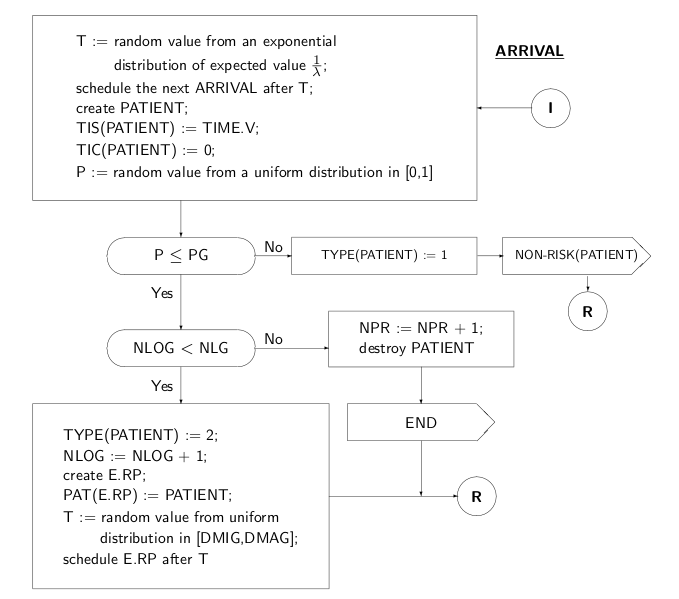
\includegraphics[width=\textwidth]{images/cap11fig41.png}
\end{figure}

\begin{figure}[H]
  \centering
  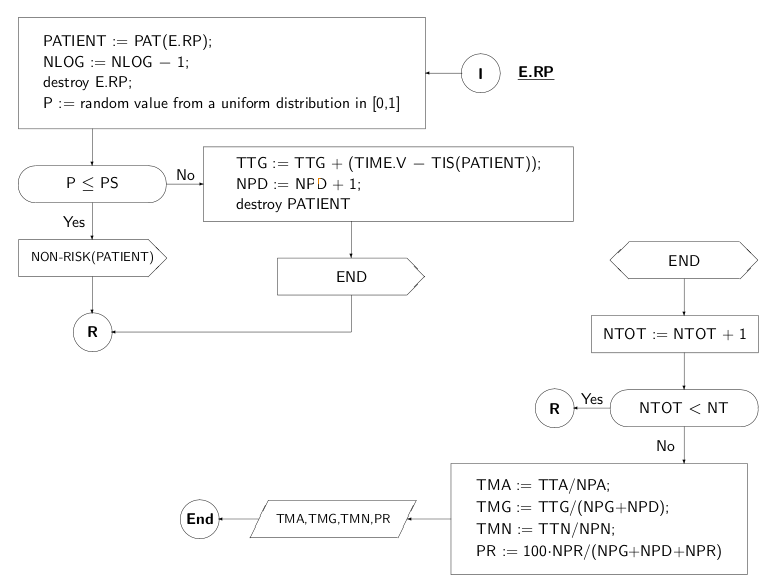
\includegraphics[width=\textwidth]{images/cap11fig42.png}
\end{figure}

\begin{figure}[H]
  \centering
  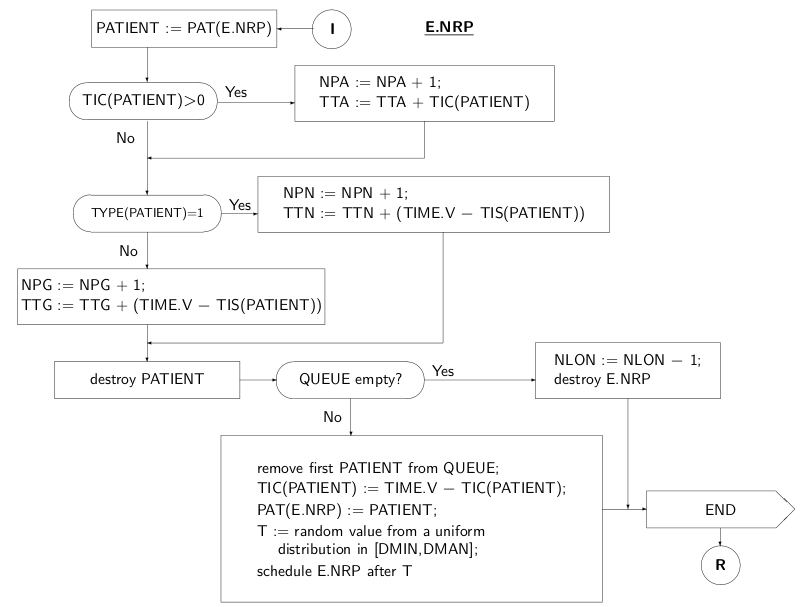
\includegraphics[width=\textwidth]{images/cap11fig43.png}
\end{figure}

\section{Esecuzione degli esperimenti}

\subsection{Debugging}

Il debugging di programmi di simulazione in genere non \`e semplice in
quanto non \`e facile individuare errori logici. Per questo motivo si
ricorre spesso a delle stampe parziali che consentano di monitorare la
creazione e distruzione di entit\`a, la creazione e l'innesco di
eventi ecc\dots

\subsection{Polarizzazione iniziale}

All'inizio della simulazione, le prime entit\`a create sono favorite
in quanto trovano le risorse libere. I valori medi raccolti dipendono
dunque dalla durata della simulazione ({\em polarizzazione
  iniziale}). Ci\`o va bene nel momento in cui si modella ad esempio
un supermercato: apre ad una certa ora e non c'\`e nessuno in
coda. Non va bene ad esempio per un ospedale che funziona a ciclo
continuo: a regime non esiste una situazione equiparabile al momento
iniziale in cui le risorse sono tutte libere. Queste alterazioni non
sono tollerabili e vanno eliminate. Per farlo esistono due metodi:

\begin{itemize}
  
\item creare uno stato iniziale attendibile. Il metodo in questione
  richiede maggior sforzo per il programmatore e l'esecuzione di vari
  test che consentano di provare l'attendibilit\`a della soluzione
  trovata, dunque viene usato raramente. Viene usato quando si
  richiede di far partire il sistema da un dato stato iniziale.

\item Iniziare da uno stato di riposo, ma dopo un certo tempo o dopo
  un certo numero di entit\`a azzerare le variabili che accumulano i
  dati statistici per eseguire la simulazione effettiva. Anche in
  questo caso occorrono delle simulazioni pilota (test) per verificare
  dopo quanto effettuare l'azzeramento.

\end{itemize}

\subsection{Sperimentazione}

Di solito si \`e interessati a provare diverse configurazioni dei
modelli di simulazione per trovare la configurazione migliore. Le
varie configurazioni vengono solitamente ottenute variando un
parametro per volta per osservare con chiarezza gli effetti prodotti.

I linguaggi di simulazione consentono, per ottenere informazioni pi\`u
accurate, di provare il sistema con diverse sequenze casuali. Per ogni
configurazione si provano pi\`u sequenze casuali e si calcola la media
delle informazioni rilevanti.

\end{document}
